\documentclass[aspectratio=169,11pt]{beamer}

\usetheme{Madrid}
\usecolortheme{default}
\setbeamertemplate{navigation symbols}{}
\setbeamertemplate{footline}[frame number]

\usepackage[T1]{fontenc}
\usepackage[utf8]{inputenc}
\usepackage{lmodern}
\usepackage{amsmath}
\usepackage{amssymb}
\usepackage{booktabs}
\usepackage{tabularx}
\usepackage{tikz}
\usepackage{listings}
\usepackage{xcolor}
\usepackage{colortbl} % for \rowcolor in tables
\usepackage{pgfplots}
\pgfplotsset{compat=1.16}
\usetikzlibrary{positioning, arrows.meta, calc, shapes.geometric, fit}
% ---------- Layout helpers for compact beamer tables/blocks ----------
\usepackage{array}
\usepackage{makecell}
\usepackage{graphicx}

\newcolumntype{Y}{>{\raggedright\arraybackslash}X}
\newcolumntype{Z}{>{\centering\arraybackslash}X}

\newcommand{\compacttable}{%
  \scriptsize
  \setlength{\tabcolsep}{2.2pt}%
  \renewcommand{\arraystretch}{1.08}%
}

\newcommand{\tightitems}{%
  \setlength{\itemsep}{1.5pt}%
  \setlength{\parsep}{0pt}%
  \setlength{\topsep}{2pt}%
}
% ---------------------------------------------------------------------
\definecolor{sdmblue}{RGB}{27, 74, 125}
\definecolor{sdmteal}{RGB}{0, 130, 127}
\definecolor{sdmorange}{RGB}{222, 123, 35}
\definecolor{sdmlight}{RGB}{244, 247, 250}
\definecolor{sdmgreen}{RGB}{67, 142, 75}
\definecolor{sdmred}{RGB}{195, 64, 64}
\definecolor{codebg}{RGB}{247, 248, 250}

\setbeamercolor{structure}{fg=sdmblue}
\setbeamercolor{palette primary}{bg=sdmblue, fg=white}
\setbeamercolor{palette secondary}{bg=sdmteal, fg=white}
\setbeamercolor{palette tertiary}{bg=sdmblue, fg=white}
\setbeamercolor{title}{bg=sdmblue, fg=white}
\setbeamercolor{subtitle}{fg=white}
\setbeamercolor{author}{fg=black!75}
\setbeamercolor{institute}{fg=black!75}
\setbeamercolor{date}{fg=black!75}
\setbeamercolor{frametitle}{bg=sdmblue!8, fg=sdmblue}
\setbeamercolor{block title}{bg=sdmblue, fg=white}
\setbeamercolor{block body}{bg=sdmlight, fg=black}
\setbeamercolor{alerted text}{fg=sdmorange}
\setbeamercolor{section in toc}{fg=sdmblue}
\setbeamercolor{section in toc shaded}{fg=black!35}

\lstset{
  basicstyle=\ttfamily\scriptsize,
  backgroundcolor=\color{codebg},
  frame=single,
  rulecolor=\color{sdmblue!30},
  columns=fullflexible,
  keepspaces=true,
  showstringspaces=false,
  breaklines=true
}

\title{Using Deep Reinforcement Learning to Solve TSP}
\subtitle{SDM-5031 Course Project Presentation}
\author{Zhao Ruojia, Ruan Zhiwen, Wu Fengyang}
\institute{Supervisor: Zhenkun Wang}
\date{Spring 2026}

\AtBeginSection[]{
  \begin{frame}{Outline}
    % \vspace{0.15cm}
    % \vspace{0.25cm}
    \tableofcontents[
      currentsection,
      sectionstyle=show/shaded,
      subsectionstyle=hide
    ]
  \end{frame}
}

\begin{document}

% =====================================================================
% Slide 1: Title / Cover
% =====================================================================
\begin{frame}[plain]
  \titlepage
\end{frame}

\section{Background and Baseline}

% =====================================================================
% Slide 2: Project overview
% =====================================================================
\begin{frame}[t]{Project Overview}
  \vspace{0.5cm}
  {\usebeamerfont{title}\color{sdmblue}\LARGE\textbf{Using Deep Reinforcement Learning to Solve TSP}\par}
  \vspace{0.1cm}
  {\large SDM-5031 Course Project --- Spring 2026\par}
  \vspace{0.4cm}
  {Zhao Ruojia, Ruan Zhiwen, Wu Fengyang\par}

  \vspace{1.0cm}
  \begin{columns}[T,totalwidth=\textwidth]
    \begin{column}{0.55\textwidth}
      \begin{block}{Headline result}
        \textbf{73.2\%} relative reduction in \texttt{avg\_aug\_gap}
        on the validation set, starting from the bundled
        3000-epoch POMO baseline.
      \end{block}
    \end{column}
    \begin{column}{0.40\textwidth}
      \begin{alertblock}{Three modules}
        \begin{itemize}
          \item distance / kNN logit bias
          \item Mixed Structured Curriculum
          \item leader-focused reward
        \end{itemize}
      \end{alertblock}
    \end{column}
  \end{columns}
  \vfill
\end{frame}

% =====================================================================
% Slide 3: Problem & Motivation
% =====================================================================
\begin{frame}{TSP, POMO Baseline}
  \begin{columns}[T,totalwidth=\textwidth]
    \begin{column}{0.55\textwidth}
      \begin{block}{Setup}
        \begin{itemize}
          \item TSP is NP-hard; POMO trains a Transformer policy on TSP-100
                with multi-rollout REINFORCE
          \item Course gives a 3000-epoch baseline checkpoint
          \item Official metric: \texttt{avg\_aug\_gap}
                (best across 8-fold augmentation)
        \end{itemize}
      \end{block}

      \begin{block}{Why this is non-trivial}
        Naive 400-epoch fine-tune barely moves the needle ---
        the baseline is already converged on uniform $[0,1]^2$ data.
      \end{block}
    \end{column}

    \begin{column}{0.42\textwidth}
      \centering
      {\scriptsize
      \setlength{\tabcolsep}{3pt}
      \renewcommand{\arraystretch}{1.15}

      \begin{tabularx}{\linewidth}{@{}>{\raggedright\arraybackslash}X c@{}}
        \toprule
        \textbf{Setting} &
        \textbf{\shortstack{val\\\texttt{avg\_aug\_gap}}} \\
        \midrule
        Baseline (3000 ep) & 2.330\% \\
        +400 ep, no modules & 1.962\% \\
        +400 ep, our three modules & 1.122\% \\
        \rowcolor{sdmblue!12}
        \textbf{+ Phase 4 size curriculum} & \textbf{0.624\%} \\
        \bottomrule
      \end{tabularx}
      }

      \vspace{0.30cm}

      {\small
      {\color{sdmorange}\textbf{Pure fine-tuning alone reduces \texttt{avg\_aug\_gap} by 0.37\%.}}\\
      {\color{sdmblue}\textbf{Three modules add another $-$0.84\%; Phase 4 adds $-$0.50\% more.}}
      }
    \end{column}
  \end{columns}
\end{frame}

\section{Three Proposed Modules}
%=========================================================
% Slide 4: Three Innovations Overview
% =====================================================================
\begin{frame}[t]{Three Modules at Three Levels of the Pipeline}
  \centering
  \vspace{-0.05cm}

  \resizebox{\linewidth}{!}{%
  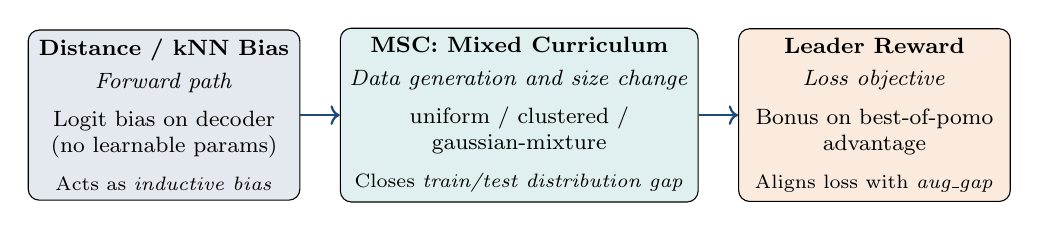
\begin{tikzpicture}[node distance=0.5cm, every node/.style={align=center, font=\footnotesize}]
    \node[draw, rounded corners, fill=sdmblue!12, minimum width=3.45cm, minimum height=2.15cm] (m2)
      {\textbf{Distance / kNN Bias}\\[0.08cm]
       \textit{Forward path}\\[0.15cm]
       Logit bias on decoder\\
       (no learnable params)\\[0.15cm]
       \scriptsize Acts as \emph{inductive bias}};

    \node[draw, rounded corners, fill=sdmteal!12, minimum width=3.45cm, minimum height=2.15cm, right=of m2] (msc)
      {\textbf{MSC: Mixed Curriculum}\\[0.08cm]
       \textit{Data generation and size change}\\[0.15cm]
       uniform / clustered /\\
       gaussian-mixture\\[0.15cm]
       \scriptsize Closes \emph{train/test distribution gap}};

    \node[draw, rounded corners, fill=sdmorange!15, minimum width=3.45cm, minimum height=2.15cm, right=of msc] (m3)
      {\textbf{Leader Reward}\\[0.08cm]
       \textit{Loss objective}\\[0.15cm]
       Bonus on best-of-pomo\\
       advantage\\[0.15cm]
       \scriptsize Aligns loss with \emph{aug\_gap}};

    \draw[->, thick, sdmblue] (m2) -- (msc);
    \draw[->, thick, sdmblue] (msc) -- (m3);
  \end{tikzpicture}%
  }

  \vspace{0.38cm}
  \begin{alertblock}{Design principle}
    \small
    Each module acts on a \textbf{different level} of the pipeline.
    They can be independently enabled / disabled, which makes ablation clean.
  \end{alertblock}
\end{frame}

% =====================================================================
% Slide 5: Why distance/kNN helps
% =====================================================================
\begin{frame}[t]{Why Distance / kNN Bias? Local Geometry Is Easy to Miss}
  \small
  \begin{columns}[T,onlytextwidth]
    \begin{column}{0.70\textwidth}
      \begin{block}{Observed failure}
        \centering
        \includegraphics[width=\linewidth,height=0.65\textheight,keepaspectratio]{picture/pomo_ood_failure.png}
      \end{block}
    \end{column}
    \hfill
    \begin{column}{0.27\textwidth}
      \begin{alertblock}{Takeaway}
        \scriptsize
        The baseline may jump across clusters while nearby nodes remain unvisited.
        Distance/kNN bias makes local candidates easier to select.
      \end{alertblock}
    \end{column}
  \end{columns}

  \vspace{0.02cm}
  % \begin{block}{kNN gives a useful candidate prior}
  %   \centering
  %   \includegraphics[width=\linewidth,height=0.20\textheight,keepaspectratio]{picture/knn_effect.png}
  % \end{block}
  \footnotetext[1]{\scriptsize
Y. L. Goh et al.,
``Hierarchical Neural Constructive Solver for Real-world TSP Scenarios,''
KDD, 2024, arXiv:2408.03585.}

\end{frame}


\begin{frame}[t]{Why Distance / kNN Bias? Local Geometry Is Easy to Miss}
  \small
  \begin{block}{Observed failure}
    \centering
    \includegraphics[width=\linewidth,height=0.5\textheight,keepaspectratio]{picture/knn_effect.png}
  \end{block}

  \begin{alertblock}{Takeaway}
    \centering
    \scriptsize
    The baseline may jump across clusters while nearby nodes remain unvisited.
    Distance/kNN bias makes local candidates easier to select.
  \end{alertblock}

  \footnotetext[1]{\scriptsize
A. Lischka, J. Wu, R. Basso, M. H. Chehreghani, and B. Kulcsár,
``Less Is More: On the Importance of Sparsification for Transformers and Graph Neural Networks for TSP,''
arXiv:2403.17159, 2024.}

\end{frame}

% =====================================================================
% Slide 5: M2 Distance/kNN Bias
% =====================================================================
\begin{frame}[t]{Distance-Aware / kNN Logit Bias}
  \small
  \begin{columns}[T,onlytextwidth]
    \begin{column}{0.55\textwidth}
      \begin{block}{Mechanism}
        At each decoding step, add a bias to the next-node logit:
        \vspace{-0.05cm}
        \[
          \ell_{ij} \leftarrow \ell_{ij}
          - \alpha \cdot \tilde{d}_{ij}
          + \beta \cdot \mathbf{1}\!\left[j \in \mathrm{kNN}(i)\right]
        \]
        \vspace{-0.15cm}
        \begin{itemize}\tightitems
          \item $\tilde{d}_{ij}$: mean-normalized Euclidean distance
          \item $\mathrm{kNN}(i)$: $k$ nearest neighbours, raw distance
          \item $\alpha = \beta = 1.0$, $k = 20$ after sweep
          \item \textbf{Zero learnable parameters}
        \end{itemize}
      \end{block}
    \end{column}
    \hfill
    \begin{column}{0.42\textwidth}
      \begin{block}{Why it helps}
        \begin{itemize}\tightitems
          \item Encoder gets only $(x,y)$; distance is not an input feature
          \item Bias injects a cheap geometric prior at the logit level
          \item Avoids architectural changes; input dim stays 2
          \item Linear warm-up in Phase 1 avoids disturbing the baseline
        \end{itemize}
      \end{block}
      \begin{alertblock}{Engineering detail}
        \scriptsize
        Bias config is embedded in the saved checkpoint and \textbf{auto-attached at test time}: no extra CLI flag required by the grader.
      \end{alertblock}
    \end{column}
  \end{columns}
\end{frame}

% =====================================================================
% Slide 6: Distance bias mechanism
% =====================================================================
\begin{frame}[t]{Distance Bias in the Current POMO Architecture}
  \small
  \centering
  \vspace{0.18cm}
  \resizebox{0.98\linewidth}{!}{%
  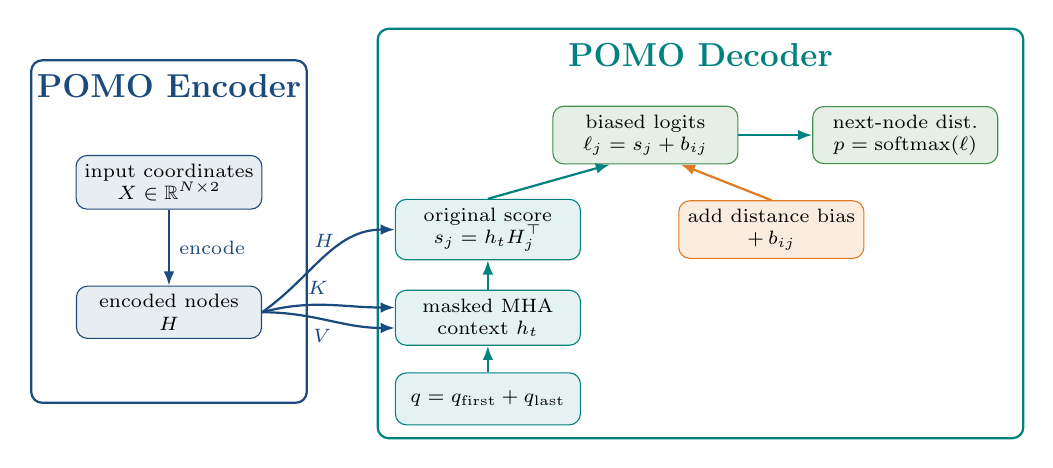
\begin{tikzpicture}[
      block/.style={draw, rounded corners, align=center, font=\scriptsize,
        minimum width=2.35cm, minimum height=0.66cm, inner sep=3pt},
      enc/.style={block, fill=sdmblue!10, draw=sdmblue},
      dec/.style={block, fill=sdmteal!10, draw=sdmteal},
      bias/.style={block, fill=sdmorange!14, draw=sdmorange},
      outnode/.style={block, fill=sdmgreen!14, draw=sdmgreen},
      arr/.style={-{Latex[length=1.8mm]}, thick, sdmblue},
      barr/.style={-{Latex[length=1.8mm]}, thick, sdmorange},
      flow/.style={-{Latex[length=1.8mm]}, thick, sdmteal}
    ]
    \draw[rounded corners, thick, sdmblue] (-5.75,-2.10) rectangle (-2.25,2.25);
    \node[font=\large\bfseries, text=sdmblue] at (-4.00,1.92) {POMO Encoder};

    \node[enc] (coords) at (-4.00,0.70) {input coordinates\\$X\in\mathbb{R}^{N\times2}$};
    \node[enc] (encoded) at (-4.00,-0.95) {encoded nodes\\$H$};
    \draw[arr] (coords) -- node[right, font=\scriptsize] {encode} (encoded);

    \draw[rounded corners, thick, sdmteal] (-1.35,-2.55) rectangle (6.85,2.65);
    \node[font=\large\bfseries, text=sdmteal] at (2.75,2.32) {POMO Decoder};

    \node[dec] (query) at (0.05,-2.05) {$q=q_{\mathrm{first}}+q_{\mathrm{last}}$};
    \node[dec] (mha) at (0.05,-1.02) {masked MHA\\context $h_t$};
    \node[dec] (score) at (0.05,0.10) {original score\\$s_j=h_tH_j^\top$};
    \node[bias] (biasrow) at (3.65,0.10) {add distance bias\\$+\,b_{ij}$};
    \node[outnode] (merge) at (2.05,1.30) {biased logits\\$\ell_j=s_j+b_{ij}$};
    \node[outnode] (prob) at (5.35,1.30) {next-node dist.\\$p=\mathrm{softmax}(\ell)$};

    \draw[flow] (query) -- (mha);
    \draw[flow] (mha) -- (score);
    \draw[flow] (score.north) -- ([xshift=-0.45cm]merge.south);
    \draw[barr] (biasrow.north) -- ([xshift=0.45cm]merge.south);
    \draw[flow] (merge) -- (prob);

    \draw[arr] (encoded.east) to[out=15,in=180]
      node[pos=0.42, above, font=\scriptsize] {$K$} ([yshift=0.13cm]mha.west);
    \draw[arr] (encoded.east) to[out=0,in=180]
      node[pos=0.45, below, font=\scriptsize] {$V$} ([yshift=-0.13cm]mha.west);
    \draw[arr] (encoded.east) to[out=35,in=180]
      node[pos=0.50, above, font=\scriptsize] {$H$} (score.west);
  \end{tikzpicture}%
  }
\end{frame}

% =====================================================================
% Slide 7: Why MSC helps
% =====================================================================
\begin{frame}[t]{Why Mixed Structured Curriculum? Training Should Resemble Testing}
  \small
  \centering
  \includegraphics[width=0.92\linewidth,height=0.60\textheight,keepaspectratio,trim=0 105 0 0,clip]{picture/msc_distribution_gap.png}

  \vspace{0.14cm}
  \begin{alertblock}{Takeaway}
    \small
    The original sampler sees only uniform random points.
    Real benchmark instances contain clusters, grids, mixtures, and other structured layouts,
    so MSC exposes the model to those patterns during fine-tuning.
  \end{alertblock}
\end{frame}

% =====================================================================
% Slide 7: MSC
% =====================================================================
\begin{frame}[t]{Mixed Structured Curriculum}
  \small
  \begin{columns}[T,onlytextwidth]
    \begin{column}{0.55\textwidth}
      \begin{block}{Why \texttt{torch.rand()} is not enough}
        Baseline POMO trains on \emph{i.i.d.\ uniform} points in $[0,1]^2$,
        but real-world instances are mostly \emph{structured}.

        \vspace{0.05cm}
        $\Rightarrow$ train / test distribution mismatch hurts generalization.
      \end{block}
      \begin{block}{Three generators, mixed per-batch}
        \begin{itemize}\tightitems
          \item \textbf{uniform}: legacy POMO sampler
          \item \textbf{clustered\_uniform}: $K\sim U[3,6]$ Gaussian clusters + small uniform background
          \item \textbf{gaussian\_mixture}: random-weight GMM, clipped to $[0,1]^2$
        \end{itemize}
      \end{block}
    \end{column}
    \hfill
    \begin{column}{0.42\textwidth}
      \begin{block}{Phase-wise mixing ratios}
        \compacttable
        \begin{tabularx}{\linewidth}{@{}Y c c c@{}}
          \toprule
                  & uniform & \makecell{clustered} & \makecell{gaussian} \\
          \midrule
          Phase 1 & 0.6     & 0.3       & 0.1      \\
          Phase 2 & 0.4     & 0.4       & 0.2      \\
          Phase 3 & 0.2     & 0.5       & 0.3      \\
          \bottomrule
        \end{tabularx}
        \par\vspace{0.16cm}
        Hard distributions are gradually emphasized.
      \end{block}
      \centering
      {\color{sdmblue}\itshape\small Closes train / test distribution gap on the validation dataset.}
    \end{column}
  \end{columns}
\end{frame}


% =====================================================================
% Slide: Size Curriculum (mixed-N training) - extension
% =====================================================================
\begin{frame}[t]{Extension: Size Curriculum (Mixed-$N$ Training)}
  \begingroup
  \fontsize{7.2pt}{8.3pt}\selectfont
  \vspace{-0.12cm}

  \begin{columns}[T,onlytextwidth]
    % ---------------- Left column ----------------
    \begin{column}{0.53\textwidth}
      \begin{block}{Motivation: OOD on large $N$}
        \begin{itemize}\tightitems
          \item Phases 1--3 are still trained at fixed $N=100$
          \item Validation dataset spans $N \in [100,300]$
          \item Large-size instances remain the main error source
          \item Goal: improve size generalization without changing the model
        \end{itemize}
      \end{block}

      \vspace{-0.04cm}
      \begin{block}{Mixed-$N$ batch sampler}
        \vspace{-0.14cm}
        \[
          N \sim \mathrm{Cat}\{100,150,200,250\},
          \qquad
          w=[1,3,3,2]
        \]
        \vspace{-0.30cm}
        \begin{itemize}\tightitems
          \item Lower weight on $N=100$: already well adapted
          \item Higher weight on $N=150,200,250$: unseen in Phases 1--3
          \item Each batch still uses a single $N$ due to tensor constraints
          \item Data generated by the same MSC samplers
        \end{itemize}
      \end{block}
    \end{column}

    \hfill

    % ---------------- Right column ----------------
    \begin{column}{0.44\textwidth}
      \begin{block}{Training setup}
        \setlength{\tabcolsep}{2.6pt}
        \renewcommand{\arraystretch}{1.00}
        \begin{tabularx}{\linewidth}{@{}Y Y@{}}
          \toprule
          \textbf{Item} & \textbf{Setting} \\
          \midrule
          Init. ckpt & Phase-3 best \\
          Epochs & 150 \\
          Episodes & 50k / epoch \\
          Learning rate & $1{\times}10^{-5} \to 1{\times}10^{-6}$ \\
          Batch size & 48 \\
          Leader reward & frozen endpoint $\gamma$ \\
          kNN bias & inherited, $k=20$ \\
          \bottomrule
        \end{tabularx}
      \end{block}

      \vspace{-0.08cm}
      \begin{alertblock}{Validation result}
        \setlength{\tabcolsep}{2.6pt}
        \renewcommand{\arraystretch}{1.00}
        \begin{tabularx}{\linewidth}{@{}Y c c@{}}
          \toprule
          \textbf{Model} & \textbf{Gap} & \textbf{Drop} \\
          \midrule
          Baseline & 2.330\% & -- \\
          Phases 1--3 & 1.122\% & $-51.8\%$ \\
          \rowcolor{sdmblue!18}
          \textbf{+ Phase 4} & \textbf{0.624\%} & \textbf{$-73.2\%$} \\
          \bottomrule
        \end{tabularx}

        \vspace{0.06cm}
        \centering
        {Phase 4 adds another \textbf{$-0.50$ percentage points}.}
      \end{alertblock}

      \vspace{-0.06cm}
      {\color{sdmblue}
      \textbf{Takeaway:} mixed-size training improves generalization to larger validation instances.}
    \end{column}
  \end{columns}
  \endgroup
\end{frame}


% =====================================================================
% Slide 7: M3 Leader-focused Reward
% =====================================================================
\begin{frame}[t]{Leader-Focused Reward}
  \small
  \begin{columns}[T,onlytextwidth]
    \begin{column}{0.55\textwidth}
      \begin{block}{Aligning loss with the test metric}
        Test metric is \textbf{best-of-pomo} under 8-fold augmentation,
        but POMO's training advantage is centred at the \emph{mean}:
        \vspace{-0.05cm}
        \[
          A_i^{\text{POMO}} = r_i - \bar{r},
          \qquad
          \mathcal{L}^{\text{POMO}} = -\mathbb{E}\!\left[A_i \log p_i\right]
        \]
      \end{block}
      \begin{block}{Leader-focused advantage: \texttt{bonus\_adv}}
        \vspace{-0.1cm}
        \[
          A_i = (r_i - \bar{r}) + \gamma\,(r_{\max} - \bar{r})
          \mathbf{1}\!\left[i = \arg\max_j r_j\right]
        \]
        \vspace{-0.2cm}
        \begin{itemize}\tightitems
          \item $\gamma$ ramps $0 \!\to\! \gamma_0 \!\to\! \gamma_1$ during Phase 3
          \item Higher $\gamma$ emphasizes the best rollout's signal
        \end{itemize}
      \end{block}
    \end{column}
    \hfill
    \begin{column}{0.42\textwidth}
      \begin{block}{Why this matters}
        \begin{itemize}\tightitems
          \item Test \texttt{aug\_gap} = $\min$ over 8 augmentations
          \item POMO rewards \emph{average} rollout performance
          \item Leader bonus \textbf{shifts gradient} to the best rollout
          \item Direct alignment with the evaluation metric
        \end{itemize}
      \end{block}
      \begin{alertblock}{Coupling with lr}
        \scriptsize
        Phase 3 ramps lr from $1\!\times\!10^{-5}$ to $5\!\times\!10^{-5}$ to give the leader signal enough push, then decays to $5\!\times\!10^{-6}$.
      \end{alertblock}
    \end{column}
  \end{columns}
\end{frame}

\section{Phased Training and Implementation}

% =====================================================================
% Slide 8: Phased Training Framework
% =====================================================================
\begin{frame}[t]{Phased Schedule --- When to Activate What}
  \centering
  \vspace{-0.05cm}
  \resizebox{\linewidth}{!}{%
  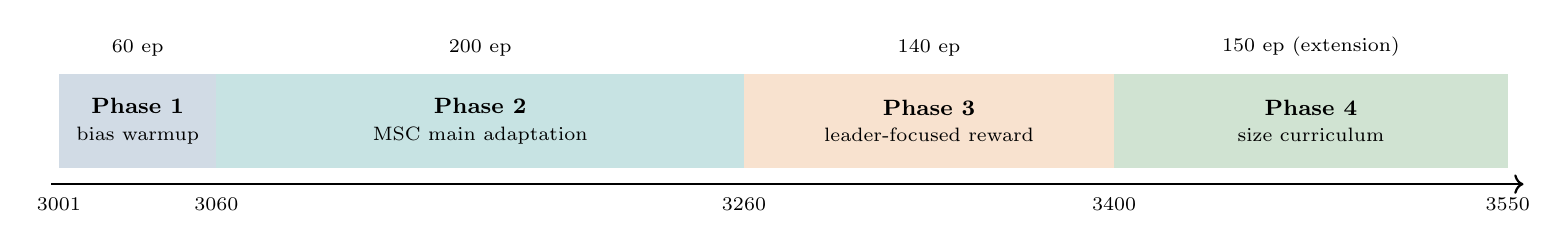
\begin{tikzpicture}[every node/.style={align=center, font=\footnotesize}]
    \fill[sdmblue!20]   (0,0)    rectangle (2.0, 1.2);
    \fill[sdmteal!22]   (2.0,0)  rectangle (8.7, 1.2);
    \fill[sdmorange!22] (8.7,0)  rectangle (13.4, 1.2);
    \fill[sdmgreen!25]  (13.4,0) rectangle (18.4, 1.2);

    \node at (1.0, 0.6)  {\textbf{Phase 1}\\\scriptsize bias warmup};
    \node at (5.35, 0.6) {\textbf{Phase 2}\\\scriptsize MSC main adaptation};
    \node at (11.05, 0.6){\textbf{Phase 3}\\\scriptsize leader-focused reward};
    \node at (15.9, 0.6) {\textbf{Phase 4}\\\scriptsize size curriculum};

    \draw[->, thick] (-0.1, -0.2) -- (18.6, -0.2);
    \node[anchor=north] at (0.0, -0.25)  {\scriptsize 3001};
    \node[anchor=north] at (2.0, -0.25)  {\scriptsize 3060};
    \node[anchor=north] at (8.7, -0.25)  {\scriptsize 3260};
    \node[anchor=north] at (13.4, -0.25) {\scriptsize 3400};
    \node[anchor=north] at (18.4, -0.25) {\scriptsize 3550};

    \node[anchor=south] at (1.0, 1.3)  {\scriptsize 60 ep};
    \node[anchor=south] at (5.35, 1.3) {\scriptsize 200 ep};
    \node[anchor=south] at (11.05, 1.3){\scriptsize 140 ep};
    \node[anchor=south] at (15.9, 1.3) {\scriptsize 150 ep (extension)};
  \end{tikzpicture}%
  }

  \vspace{0.30cm}
  \begin{columns}[T,onlytextwidth]
    \begin{column}{0.235\textwidth}
      \begin{block}{Phase 1 --- bias adapter}
        \scriptsize
        bias on, linear warm-up $0\!\to\!1$\\
        MSC on, uniform-heavy ratios\\
        leader OFF, lr $=1\!\times\!10^{-5}$
      \end{block}
    \end{column}
    \hfill
    \begin{column}{0.235\textwidth}
      \begin{block}{Phase 2 --- MSC main}
        \scriptsize
        bias on at full strength\\
        MSC on, balanced ratios\\
        leader OFF, lr $=1\!\times\!10^{-5}$
      \end{block}
    \end{column}
    \hfill
    \begin{column}{0.235\textwidth}
      \begin{block}{Phase 3 --- leader}
        \scriptsize
        bias on, MSC hard-leaning\\
        leader ON, $\gamma$ ramp\\
        lr $5\!\times\!10^{-5}\!\to\!5\!\times\!10^{-6}$
      \end{block}
    \end{column}
    \hfill
    \begin{column}{0.235\textwidth}
      \begin{block}{Phase 4 --- size curriculum}
        \scriptsize
        bias inherited, MSC on\\
        $N\!\sim\!\{100,150,200,250\}$\\
        leader frozen, lr $1\!\times\!10^{-5}\!\to\!1\!\times\!10^{-6}$
      \end{block}
    \end{column}
  \end{columns}

  \vspace{0.10cm}
  {\scriptsize\color{sdmblue}\textbf{Single \texttt{finetune\_phased.py} entry $\Rightarrow$ all ablations share the same code path.}}
\end{frame}

% =====================================================================
% Slide 9: implementation
% =====================================================================
\begin{frame}[fragile,t]{Implementation: Distance / kNN Logit Bias}
  \small
  \begin{columns}[T,onlytextwidth]
    \begin{column}{0.60\textwidth}
      \begin{block}{1. Cache geometry once per problem batch}
      \begin{lstlisting}[language=Python,basicstyle=\ttfamily\tiny]
diff = problems[:, :, None, :] - problems[:, None, :, :]
dist = (diff * diff).sum(-1).clamp(min=0.0).sqrt()
dist_nodiag = dist.masked_fill(eye, float("nan"))
mean = torch.nanmean(dist_nodiag, dim=(1, 2), keepdim=True)
self._norm_dist = dist / mean.clamp(min=1e-8)
sorted_dist = dist.masked_fill(eye, float("inf"))
_, nn_idx = sorted_dist.topk(k, dim=-1, largest=False)
mask[batch_idx, row_idx, nn_idx] = True
self._knn_mask = mask
      \end{lstlisting}
      \end{block}
      \begin{block}{2. Gather the live row and add it to logits}
      \begin{lstlisting}[language=Python,basicstyle=\ttfamily\tiny]
dist_rows = self._norm_dist.gather(dim=1, index=idx)
bias = bias - scale * dist_rows
knn_rows = self._knn_mask.gather(dim=1, index=idx)
bias = bias + knn_bias_value * knn_rows
return bias
      \end{lstlisting}
      \end{block}
    \end{column}
    \hfill
    \begin{column}{0.36\textwidth}
      \begin{block}{POMO hook}
      \begin{lstlisting}[language=Python,basicstyle=\ttfamily\tiny]
self.decoder.set_bias_module(module)
self.distance_bias_module.prepare(reset_state.problems)

score_clipped = logit_clipping * torch.tanh(score_scaled)
score_clipped = score_clipped + bias
score_masked = score_clipped + ninf_mask
probs = F.softmax(score_masked, dim=2)
      \end{lstlisting}
      \end{block}
      \begin{alertblock}{Interpretation}
        \scriptsize
        \begin{itemize}\tightitems
          \item \texttt{prepare()} does pairwise work once; the decoder only gathers live rows.
          \item Bias is added before \texttt{ninf\_mask}, so visited nodes remain impossible.
        \end{itemize}
      \end{alertblock}
    \end{column}
  \end{columns}
\end{frame}

% =====================================================================
% Slide 10: MSC implementation
% =====================================================================
\begin{frame}[fragile,t]{Implementation: Mixed Structured Curriculum}
  \small
  \begin{columns}[T,onlytextwidth]
    \begin{column}{0.60\textwidth}
      \begin{block}{1. Phase schedule chooses the mixture}
      \begin{lstlisting}[language=Python,basicstyle=\ttfamily\tiny]
DEFAULT_PHASE_RECIPE = {
    "phase1": {"msc_ratios": {"uniform": 0.6,
        "clustered_uniform": 0.3, "gaussian_mixture": 0.1}},
    "phase2": {"msc_ratios": {"uniform": 0.4,
        "clustered_uniform": 0.4, "gaussian_mixture": 0.2}},
    "phase3": {"msc_ratios": {"uniform": 0.2,
        "clustered_uniform": 0.5, "gaussian_mixture": 0.3}},
}
      \end{lstlisting}
      \end{block}
      \begin{block}{2. Sampler builds one mixed training batch}
      \begin{lstlisting}[language=Python,basicstyle=\ttfamily\tiny]
ratios = get_stage_ratios(stage_idx, curriculum_cfg)
counts = sample_distribution_types(batch_size, ratios)
problems = _build_problems_with_counts(problem_size, counts, config)
perm = torch.randperm(problems.size(0), device=problems.device)
problems = problems.index_select(0, perm)
      \end{lstlisting}
      \end{block}
    \end{column}
    \hfill
    \begin{column}{0.36\textwidth}
      \begin{block}{Generator dispatch}
      \begin{lstlisting}[language=Python,basicstyle=\ttfamily\tiny]
if n_uniform > 0:
    chunks.append(generate_uniform(...))
if n_clu > 0:
    chunks.append(generate_clustered_uniform(...))
if n_gm > 0:
    chunks.append(generate_gaussian_mixture(...))
return torch.cat(chunks, dim=0)
      \end{lstlisting}
      \end{block}
      \begin{alertblock}{Interpretation}
        \scriptsize
        \begin{itemize}\tightitems
          \item We change what the model sees, not the encoder/decoder.
          \item Ratios move from uniform-heavy to clustered and multi-modal data.
        \end{itemize}
      \end{alertblock}
    \end{column}
  \end{columns}
\end{frame}

% =====================================================================
% Slide 11: M3 implementation
% =====================================================================
\begin{frame}[fragile,t]{Implementation: Leader-Focused Reward}
  \small
  \begin{columns}[T,onlytextwidth]
    \begin{column}{0.60\textwidth}
      \begin{block}{1. Trainer swaps the loss only when enabled}
      \begin{lstlisting}[language=Python,basicstyle=\ttfamily\tiny]
log_prob = prob_list.log().sum(dim=2)

if self.leader_cfg is not None:
    loss_mean, leader_stats = compute_leader_loss(
        reward, log_prob, self.leader_cfg)
else:
    advantage = reward - reward.float().mean(dim=1, keepdims=True)
    loss_mean = (-advantage * log_prob).mean()
      \end{lstlisting}
      \end{block}
      \begin{block}{2. Best rollout receives extra advantage}
      \begin{lstlisting}[language=Python,basicstyle=\ttfamily\tiny]
baseline = reward.float().mean(dim=1, keepdim=True)
base_adv = reward - baseline
leader_idx = reward.float().argmax(dim=1)
leader_adv = reward[batch_arange, leader_idx] - baseline.squeeze(1)
bonus[batch_arange, leader_idx] = gamma * leader_adv
loss = -((base_adv + bonus) * log_prob).mean()
      \end{lstlisting}
      \end{block}
    \end{column}
    \hfill
    \begin{column}{0.36\textwidth}
      \begin{block}{Phase-3 strength ramp}
      \begin{lstlisting}[language=Python,basicstyle=\ttfamily\tiny]
if in_phase <= rampup_epochs:
    ramp = in_phase / rampup_epochs
    cur_gamma = gamma_start + (gamma_target - gamma_start) * ramp
else:
    cur_gamma = gamma_target + (gamma_final - gamma_target) * tail_frac
trainer.leader_cfg["leader_gamma"] = float(cur_gamma)
      \end{lstlisting}
      \end{block}
      \begin{alertblock}{Interpretation}
        \scriptsize
        \begin{itemize}\tightitems
          \item The metric uses the best POMO rollout; this loss gives it extra gradient.
          \item The ramp avoids giving the new objective full weight immediately.
        \end{itemize}
      \end{alertblock}
    \end{column}
  \end{columns}
\end{frame}

% =====================================================================
% Slide 11b: Size Curriculum implementation
% =====================================================================
\begin{frame}[fragile,t]{Implementation: Size Curriculum (Mixed-$N$ Training)}
  \small
  \begin{columns}[T,onlytextwidth]
    \begin{column}{0.60\textwidth}
      \begin{block}{1. CLI flags assemble the $N$-sampler config}
      \begin{lstlisting}[language=Python,basicstyle=\ttfamily\tiny]
n_vals = [int(x) for x in args.n_values.split(',')]
n_wts = [float(x) for x in args.n_weights.split(',')] \
        if args.n_weights else None
trainer_params['n_sampler_cfg'] = {
    'enabled': True,
    'n_values': n_vals,   # e.g. [100, 150, 200, 250]
    'weights':  n_wts,    # e.g. [1, 3, 3, 2]
}
      \end{lstlisting}
      \end{block}
      \begin{block}{2. Per-batch $N$ resample before \texttt{load\_problems}}
      \begin{lstlisting}[language=Python,basicstyle=\ttfamily\tiny]
if self.n_sampler_cfg and self.n_sampler_cfg['enabled']:
    n = random.choices(n_values, weights=n_weights, k=1)[0]
    self.env.problem_size = int(n)
    self.env.pomo_size    = int(n)
self.env.load_problems(batch_size, epoch=epoch,
                       total_epochs=self.trainer_params['epochs'],
                       msc_config=self.msc_cfg)
      \end{lstlisting}
      \end{block}
    \end{column}
    \hfill
    \begin{column}{0.36\textwidth}
      \begin{block}{Why mutate the env in place}
      \begin{lstlisting}[language=Python,basicstyle=\ttfamily\tiny]
# load_problems regenerates BATCH_IDX,
# POMO_IDX and ninf_mask using the new
# problem_size / pomo_size, so the
# whole rollout works at the sampled N
# without rebuilding the env.
      \end{lstlisting}
      \end{block}
      \begin{alertblock}{Interpretation}
        \scriptsize
        \begin{itemize}\tightitems
          \item One $N$ per batch (tensor shapes are fixed within a batch); $N$ varies across batches.
          \item Reuses the same MSC samplers (uniform / clustered / GMM); only the size axis is added.
          \item Encoder / decoder weights, bias module, and leader loss are all unchanged.
        \end{itemize}
      \end{alertblock}
    \end{column}
  \end{columns}
\end{frame}



\section{Results and Discussion}

% =====================================================================
% Slide 12: Main result
% =====================================================================
\begin{frame}[t]{Main Result --- 73.2\% Relative Improvement}
  \begin{columns}[T,onlytextwidth]
    \begin{column}{0.55\textwidth}
      \centering
      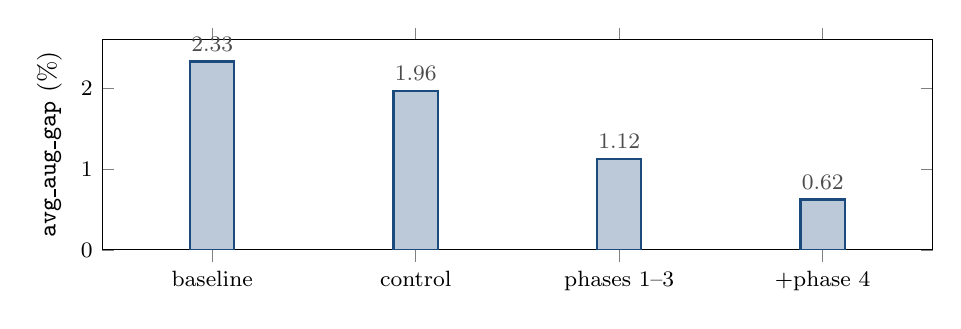
\begin{tikzpicture}
        \begin{axis}[
          ybar,
          width=\linewidth, height=4.25cm,
          ymin=0, ymax=2.6,
          ylabel={\small \texttt{avg\_aug\_gap} (\%)},
          symbolic x coords={baseline, control, phases 1--3, +phase 4},
          xtick=data,
          x tick label style={font=\footnotesize},
          y tick label style={font=\footnotesize},
          bar width=16pt,
          enlarge x limits=0.18,
          nodes near coords,
          nodes near coords style={font=\footnotesize, color=black!70},
          axis line style={-}
        ]
          \addplot[fill=sdmblue!30, draw=sdmblue, thick] coordinates {(baseline,2.330) (control,1.962) (phases 1--3,1.122) (+phase 4,0.624)};
        \end{axis}
      \end{tikzpicture}
      \par\vspace{-0.05cm}
      {\footnotesize Validation set: 10 instances, $N \in [100, 300]$}
    \end{column}
    \hfill
    \begin{column}{0.42\textwidth}
      \begin{block}{Key numbers}
        \compacttable
        \begin{tabularx}{\linewidth}{@{}Y r r@{}}
          \toprule
                          & val    \\
          \midrule
          baseline        & 2.330  \\
          control         & 1.962  \\
          phases 1--3     & 1.122  \\
          \rowcolor{sdmblue!12}
          \textbf{+ phase 4} & \textbf{0.624}  \\
          \midrule
          relative drop   & \textbf{$-$73.2\%}  \\
          \bottomrule
        \end{tabularx}
      \end{block}

      \vspace{0.08cm}
      \begin{alertblock}{Conclusion}
        \scriptsize
         relative drop is 73.2\% on val.
      \end{alertblock}
    \end{column}
  \end{columns}
\end{frame}

% =====================================================================
% Slide 9: Performance by N bucket
% =====================================================================
\begin{frame}[t]{How Does Performance Scale with $N$?}
  \begin{columns}[T,onlytextwidth]
    \begin{column}{0.55\textwidth}
      \centering
      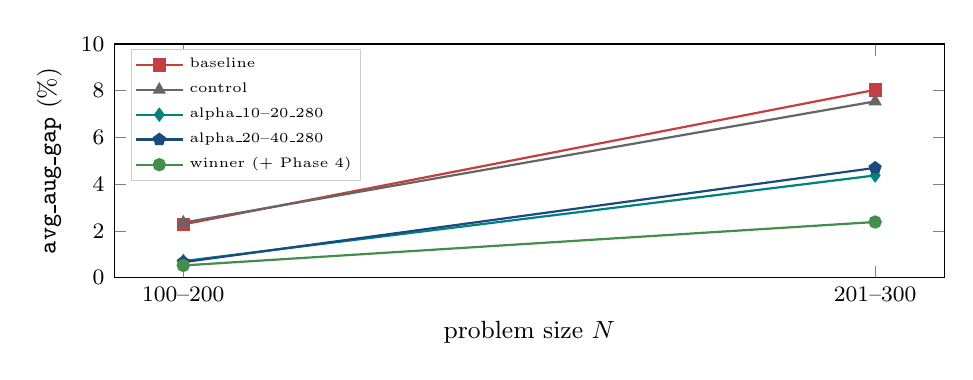
\begin{tikzpicture}
        \begin{axis}[
          width=\linewidth, height=4.55cm,
          xlabel={\small problem size $N$},
          ylabel={\small \texttt{avg\_aug\_gap} (\%)},
          symbolic x coords={100--200, 201--300},
          xtick=data,
          x tick label style={font=\footnotesize},
          y tick label style={font=\footnotesize},
          legend style={
            font=\tiny,
            at={(0.02,0.98)},
            anchor=north west,
            fill=white,
            draw=black!20,
            inner sep=1.2pt
          },
          legend cell align=left,
          ymin=0, ymax=10,
          mark size=2pt,
          axis line style={-}
        ]
          \addplot[mark=square*, color=sdmred, thick] coordinates {(100--200,2.283)(201--300,8.039)};
          \addlegendentry{baseline}
          \addplot[mark=triangle*, color=black!60, thick] coordinates {(100--200,2.359)(201--300,7.546)};
          \addlegendentry{control}
          \addplot[mark=diamond*, color=sdmteal, thick] coordinates {(100--200,0.713)(201--300,4.378)};
          \addlegendentry{alpha\_10--20\_280}
          \addplot[mark=pentagon*, color=sdmblue, thick] coordinates {(100--200,0.666)(201--300,4.702)};
          \addlegendentry{alpha\_20--40\_280}
          \addplot[mark=*, color=sdmgreen, thick] coordinates {(100--200,0.527)(201--300,2.386)};
          \addlegendentry{winner (+ Phase 4)}
        \end{axis}
      \end{tikzpicture}
      \par\vspace{-0.05cm}
      {\footnotesize Validation dataset, $N \in [100, 300]$}
    \end{column}
    \hfill
    \begin{column}{0.42\textwidth}
      \begin{block}{Best per bucket}
        \compacttable
        \begin{tabularx}{\linewidth}{@{}Y Y@{}}
          \toprule
          $N$-bucket & winner \\
          \midrule
          \makecell[l]{$[100,200]$\\[-1pt]\scriptsize in-dist}
            & \makecell[l]{\textbf{Phase 4 (mixed-$N$)}\\[-1pt]\scriptsize 0.527} \\
          \makecell[l]{$[201,300]$\\[-1pt]\scriptsize OOD}
            & \makecell[l]{\textbf{Phase 4 (mixed-$N$)}\\[-1pt]\scriptsize 2.386} \\
          \bottomrule
        \end{tabularx}
      \end{block}
      \begin{alertblock}{Observation}
        \scriptsize
        Phase 4 mixed-$N$ wins both buckets and \textbf{nearly halves the OOD gap} ($4.7\!\to\!2.4$). Among phases 1--3, lower leader $\alpha$ helps OOD $\Rightarrow$ \textbf{size-generalization trade-off}; detailed analysis on slide \pageref{fig:size-gen-tradeoff}.
      \end{alertblock}
    \end{column}
  \end{columns}
\end{frame}

% =====================================================================
% Slide 10: Hyperparameter Sensitivity
% =====================================================================
\begin{frame}[t]{Hyperparameter Sensitivity}
  \begin{columns}[T,onlytextwidth]
    \begin{column}{0.31\textwidth}
      \begin{block}{kNN $k$}
        \compacttable
        \begin{tabularx}{\linewidth}{@{}Y r@{}}
          \toprule
          $k$ & val gap \\
          \midrule
          \textbf{20} & \textbf{1.122} \\
          30          & 1.307 \\
          \bottomrule
        \end{tabularx}
        \par\vspace{0.10cm}
        {\scriptsize $k=20$ is the stable winner.}
      \end{block}
    \end{column}
    \hfill
    \begin{column}{0.31\textwidth}
      \begin{block}{leader $\alpha$}
        \compacttable
        \begin{tabularx}{\linewidth}{@{}Y c c@{}}
          \toprule
          $\alpha$ & val & \makecell{OOD\\$N>200$} \\
          \midrule
          $10\!\to\!20$ & 1.181 & \textbf{best} \\
          \textbf{$20\!\to\!40$} & \textbf{1.122} & mid \\
          $40\!\to\!60$ & 1.184 & worse \\
          \bottomrule
        \end{tabularx}
        \par\vspace{0.10cm}
        {\scriptsize U-shape on val; low $\alpha$ wins OOD.}
      \end{block}
    \end{column}
    \hfill
    \begin{column}{0.31\textwidth}
      \begin{block}{Phase 3 length}
        \compacttable
        \begin{tabularx}{\linewidth}{@{}Y c c@{}}
          \toprule
          ep & val & \makecell{valid\\$N\leq200$} \\
          \midrule
          140 & 1.122 & 0.725 \\
          \textbf{280} & \textbf{1.117} & \textbf{0.684} \\
          \bottomrule
        \end{tabularx}
        \par\vspace{0.10cm}
        {\scriptsize Doubling helps in-dist.; marginal on OOD.}
      \end{block}
    \end{column}
  \end{columns}

  \vspace{0.22cm}
  \begin{alertblock}{Three knobs, three different stories}
    \scriptsize
    kNN-$k$ is robust; leader-$\alpha$ is U-shaped \textbf{and} OOD-dependent; extra Phase 3 epochs mainly help in-distribution.
  \end{alertblock}
\end{frame}

% =====================================================================
% Slide 11: Ablation
% =====================================================================
\begin{frame}[t]{Module Contribution --- Where Does the Gain Come From?}
  \begin{columns}[T,onlytextwidth]
    \begin{column}{0.54\textwidth}
      \compacttable
      \begin{tabularx}{\linewidth}{@{}Y c c@{}}
        \toprule
        Configuration & \makecell{val\\gap} & \makecell{$\Delta$ vs\\control} \\
        \midrule
        baseline (3000 ep)            & 2.330 & --- \\
        \rowcolor{sdmlight}
        control (+400 ep, 0 modules)  & \textbf{1.962} & 0 \\
        \midrule
        bias\_only         & 1.95  & $-$0.27 \\
        msc\_only           & 1.72  & $-$0.27 \\
        leader\_only       & 1.55  & $-$0.41 \\
        \midrule
        \rowcolor{sdmblue!12}
        \textbf{all\_three}           & \textbf{1.122} & \textbf{$-$0.84} \\
        \bottomrule
      \end{tabularx}

      \par\vspace{0.14cm}

    \end{column}
    \hfill
    \begin{column}{0.43\textwidth}
      \begin{block}{Two clean facts}
        \small
        \begin{itemize}\tightitems
          \item Pure 400-epoch fine-tune buys only \textbf{0.37\%} on val: the baseline is already converged.
          \item Three modules together buy another \textbf{0.84\%}: twice the pure fine-tune effect.
        \end{itemize}
      \end{block}
      \begin{alertblock}{Why this matters}
        \scriptsize
        The \texttt{control} row \textbf{rules out the ``it's just 400 more epochs'' hypothesis}. Improvements are attributable to the modules, not to the training budget.
      \end{alertblock}
    \end{column}
  \end{columns}
\end{frame}

% =====================================================================
% Slide 12: Key Finding
% =====================================================================
\begin{frame}[t]{Key Finding --- The Size-Generalization Trade-off}
  \label{fig:size-gen-tradeoff}
  \begin{columns}[T,onlytextwidth]
    \begin{column}{0.55\textwidth}
      \centering
      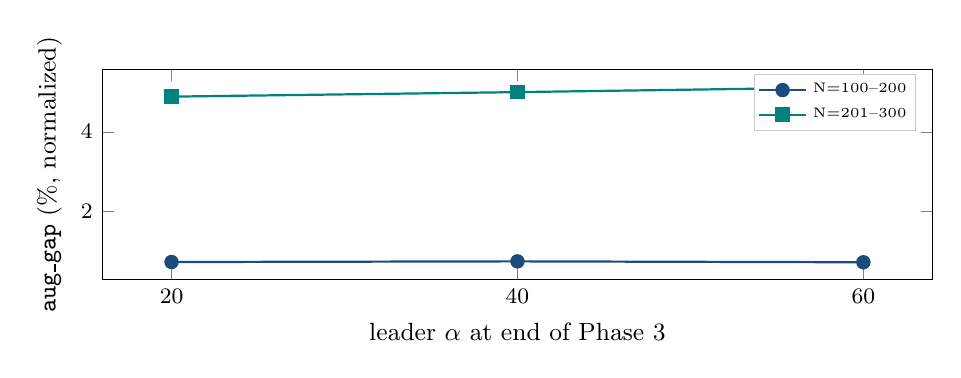
\begin{tikzpicture}
        \begin{axis}[
          width=\linewidth, height=4.25cm,
          xlabel={\small leader $\alpha$ at end of Phase 3},
          ylabel={\small \texttt{aug\_gap} (\%, normalized)},
          xtick={20, 40, 60},
          x tick label style={font=\footnotesize},
          y tick label style={font=\footnotesize},
          legend style={
            font=\tiny,
            at={(0.98,0.98)},
            anchor=north east,
            fill=white,
            draw=black!20,
            inner sep=1.2pt
          },
          mark size=2.2pt,
          axis line style={-}
        ]
          \addplot[mark=*, color=sdmblue, thick]
            coordinates {(20, 0.708)(40, 0.725)(60, 0.702)};
          \addlegendentry{N=100--200}
          \addplot[mark=square*, color=sdmteal, thick]
            coordinates {(20, 4.891)(40, 5.005)(60, 5.130)};
          \addlegendentry{N=201--300}
        \end{axis}
      \end{tikzpicture}
    \end{column}
    \hfill
    \begin{column}{0.42\textwidth}
      \begin{block}{What the curves say}
        \small
        \begin{itemize}\tightitems
          \item \textbf{Higher $\alpha$}: more aggressive best-of-pomo optimization
          \item In-distribution ($N\!\leq\!200$): U-shape, mild differences
          \item OOD ($N\!>\!200$): \textbf{lower $\alpha$ clearly better}
        \end{itemize}
      \end{block}
      \begin{alertblock}{Interpretation}
        \scriptsize
        Strong leader bonus \emph{over-specializes} to the training distribution, at the cost of OOD generalization.
      \end{alertblock}
    \end{column}
  \end{columns}

  \vspace{0.10cm}
  \centering
  {\small\color{sdmblue}\textit{Practical: choose $\alpha$ to match the assumed test-set size distribution.}}
\end{frame}

% =====================================================================
% Slide 13: Limitations & Conclusion
% =====================================================================
\begin{frame}[t]{Limitations and Conclusion}
  \footnotesize
  \begin{block}{Conclusion}
    \begin{enumerate}\tightitems
      \item Three independent modules under a phased schedule yield \textbf{51.8\%} \texttt{avg\_aug\_gap} reduction on val.
      \item Phase 4 size curriculum (mixed-$N$ sampling over $\{100,150,200,250\}$) extends fine-tuning to unseen sizes and lifts the total reduction to \textbf{73.2\%}, addressing the large-$N$ error tail.
      \item New observation: \textbf{size-OOD trade-off} in leader-focused reward strength.
      \item Engineering: ckpt-embedded \texttt{bias\_cfg} makes standard \texttt{test.py} produce the trained behaviour with zero extra flags.
    \end{enumerate}
  \end{block}

  \centering
  \vspace{0.30cm}
  {\large\color{sdmblue}\textbf{Thank you. Questions?}}
\end{frame}

% =====================================================================
% Slide 16: References
% =====================================================================
\begin{frame}[t]{References}
  \scriptsize
  \setbeamertemplate{bibliography item}{\insertbiblabel}
  \renewcommand{\newblock}{}

  \begin{thebibliography}{99}

    \bibitem{hncs}
    Y. L. Goh, Z. Cao, Y. Ma, Y. Dong, M. H. Dupty, and W. S. Lee,
    ``Hierarchical Neural Constructive Solver for Real-world TSP Scenarios,''
    \emph{arXiv preprint arXiv:2408.03585}, 2024.

    \bibitem{sparsification-tsp}
    A. Lischka, J. Wu, R. Basso, M. H. Chehreghani, and B. Kulcsár,
    ``Less Is More: On the Importance of Sparsification for Transformers and Graph Neural Networks for TSP,''
    \emph{arXiv preprint arXiv:2403.17159}, 2024.

    \bibitem{amdkd}
    J. Bi, Y. Ma, J. Wang, Z. Cao, J. Chen, Y. Sun, and Y. M. Chee,
    ``Learning Generalizable Models for Vehicle Routing Problems via Knowledge Distillation,''
    \emph{arXiv preprint arXiv:2210.07686}, 2022.

    \bibitem{distance-aware-reshaping}
    Y. Wang, Y.-H. Jia, W.-N. Chen, and Y. Mei,
    ``Distance-aware Attention Reshaping: Enhance Generalization of Neural Solver for Large-scale Vehicle Routing Problems,''
    \emph{arXiv preprint arXiv:2401.06979}, 2024.

  \end{thebibliography}
\end{frame}
\end{document}
